\section{Speech}
\label{sect:speech}
Die Sprachproduktion beim menschlichen Körper besteht aus drei Teilen: 1. dem supraglottale Sprachtrakt, 2. dem kehlkopf und 3. dem subglottalem System (teil davon ist die Lunge). Die Lunge und der Kehlkopf werden dabei über motorische Bewegung angeregt. Genauer gesagt, die Lunge stellt die Luft bereit, welche vom Kehlkopf benötigt wird um angeregt zu werden. Die Lunge und der Kehlkopf zusammen sorgen somit für die \textit{Anregung}.
Je nach ''Form'' des Vokaltrakts (Rachen-, Mund- und Nasenraum) kommt es durch die Anregung zu einer anderen \textit{Artikulation}. Dabei werden Töne erzeugt und ''ausgegeben''. Aneinander gereihte Töne ergeben dadurch Sprache.
Die verschiedenen Töne produzieren verschiedene Spektrale. Für bestimmte Laute bzw. Vokale lassen sich typische Muster im Spektralbereich finden und somit die Vokale unterscheiden.

\subsection{Speech Recognition}
\label{ssect:speech-recognition}
\begin{figure}[h]
\centering
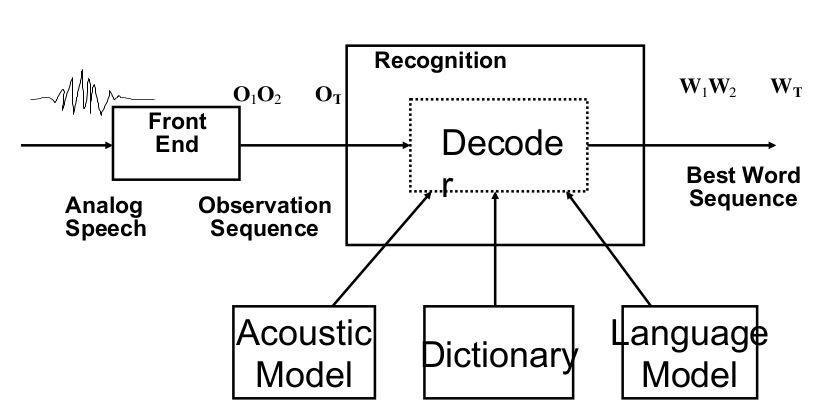
\includegraphics[scale=0.45]{komponenten-speech-recognition}
\label{graph:komponenten-speech-recognition}
\caption{Komponenten eines Sprach Erkenners}
\end{figure}
Auf dem obigen Bild sind die einzelnen Komponenten eines Sprach Erkenners zu sehen. Links kommts das \textit{analoge Signal} in das Front End rein und wird digitalisiert. Dazu wird es mittels Fouriertransformation in den Spektralbereich umgewandelt. Aus dem Frontend kommt die \textit{observation sequence} heraus und wird an den \textit{Decoder} weitergegeben. Im Decoder passiert die eigentliche Sprach Erkennung. Dazu wird ein \textit{acoustic model}, ein \textit{dictionary} und ein \textit{language model} verwendet. Die einzelnen Komponenten werden wir uns später noch genauer anschauen. Der Decoder gibt am Ende die \textit{best word sequence} aus.
Das Ziel des Sprach Erkenners ist es aus einer gegebenen akkustichen Daten $A = a_1, a_2, ..., a_k$ die Wortsequenz $W = w_1, w_2, ..., w_n$ zu finden, welche die Wahrscheinlichkeit $P(W|A)$ maximiert. Dazu brauchen wir die \textit{Bayes Regel}:
\[
P(W|A) = \frac{P(A|W) \cdot P(W)}{P(A)}
\]
P(W|A) ist das \textit{acoustic model}, P(W) ist das \textit{language model} und P(A) ist konstant für einen ganzen Satz.

\subsection{Acoustic Model}
\label{ssect:acoustic-model}

\subsubsection{Hidden Markov Model}
\label{sssect:hidden-markov-model}
Elements:
\begin{itemize}
	\item states: $S = \langle S_0, S_1, ..., S_N\rangle$
	\item transition probabilities: $P(q_t = S_i | q_{t-1} = S_j) = aji$
	\item emission probabilities: $P(y_t = O_k | q_t = S_j) = b_j(k)$
\end{itemize}
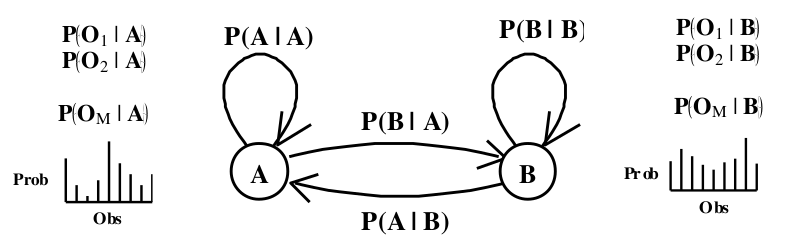
\includegraphics[scale=0.45]{hhm-example}
In der Spracherkennung spiegeln die States die phonetischen Zustände wieder (genauer gesagt besteht jedes Phonem aus drei Zuständen: beginning, middle und end). Der Decoder sucht hierbei den besten Pfad zwischen den Modellen und der Sprache.
Um die Emissionswahrscheinlichkeit zu approximieren können neben HMMs alternative Methoden verwendet werden:
\begin{itemize}
	\item Mixture of Gaussians Networks
	\item Neural Networks
	\item Hierarchies of Neural Networks
\end{itemize}

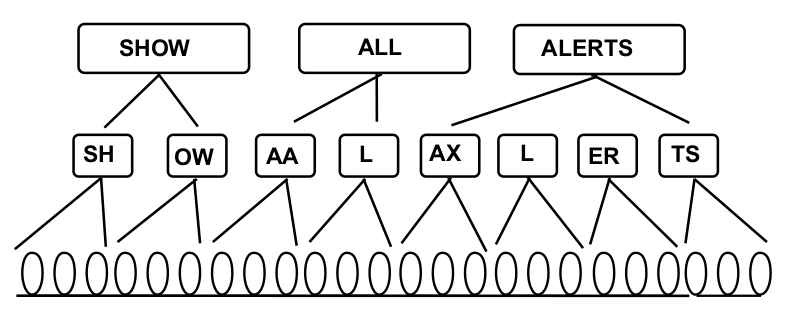
\includegraphics[scale=0.5]{alignment-phoneme-sprache}
Die Wörter werden zerlegt in Phoneme und die Phoneme in Zustände.

\subsubsection{Time Delay Neural Network (TDNN)}
\label{sssect:TDNN}
Ein \textit{time delay neural netwrok} ist eine spezielle Art von neuronalem Netz, welches \textit{time invariant} ist. Es besteht aus einem Input Layer, mehreren Hidden Layers und einem Output Layer.
Als Eingabe dient eine Matrix welche \textit{mel-scaled} ist. Die x-Achse spiegelt die Zeit wider, die y-Achse die Frequenz. Der erste Hidden Layer erhält als Eingabe ein 16 x 3 Ausschnitt der Eingabe, jeweils verschoben in der x-Richtung. Somit überlappen sich die Eingaben für den ersten Hidden Layer. Im Hidden Layer wird ebenfalls ein Fenster drüber gelegt und einem weiteren Hidden Layer als Input gegeben. Im Output Layer wird auf einzelne Buchstaben gemappt. Das bedeutet ein TDNN kann ein Muster in einem Signal finden egal wo es sich befindet. Alles was wir wissen ist, dass es darin vorkommt.
Im letzten Hidden Layer werden horizontal die Aktivierungen der Neuronen angeschaut und daraus bestimmt, welches Phonem vorgekommen ist. Der letze Hidden Layer wird auch als \textit{phoneme layer bezeichnet}. Jedoch bezieht sich das TDNN in unserem Fall auf einzelne Phoneme, jedoch werden Wörter aus mehreren Phonemen gebildet. Siehe dazu \ref{sssect:MS-TDNN}.
TDNN sind \textit{convolutional networks} mit einer festen Größe. Dies ist beim Übergang zwischen den Schichten zu sehen. Convolutional neuronale Netze werden in der Bildverarbeitung verwendet. Hierbei ist es so, dass z.B. Straßenschilder aufgenommen, aber nicht immer an der selben Stelle im Bild sind.\\
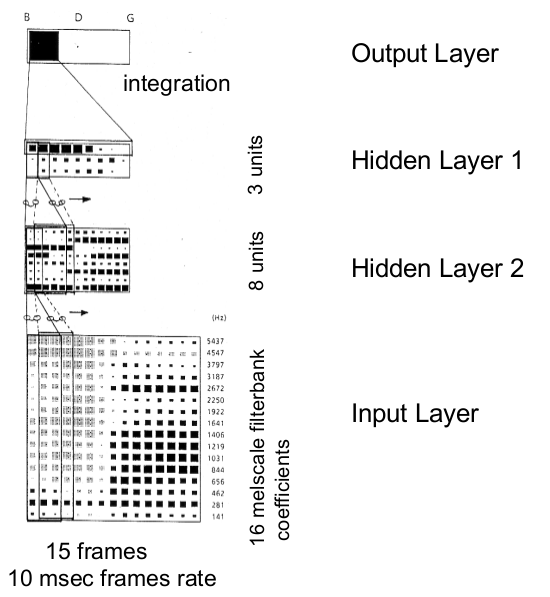
\includegraphics[scale=0.5]{tdnn}
Eine Erweiterung der TDNN stellen die \textit{frequency shifting TDNN (FSTDNN)} dar. Diese Netze sind shift invaraint in zwei Dimensionen. Das bedeute nicht nur Zeitinvariant sondern auf Frequenzinvariant. Normalerweise wird ein Netz auf eine Person trainiert und die Fehlerrate steigt, sobald eine andere Person das Netz benutzt. Die Frequenzinvarianz sorgt dafür, dass Männer, Frauen oder Kinder das selbe Nezt benutzen können und die Fehlerrate verändert sich nur gering. Dies nennt sich auch \textit{Multi-Speaker Phoneme Recognition}.
Darüber hinaus gibt es noch das Problem des Echo / der Verhallung. Wenn kein Mikrofon direkt am Mund getragen wird, wird das Signal verrauscht / verschmiert. Die Verhallung ist immer unterschiedlich und man kann kein Netz für jeden Raum bauen. Bei der Verhallung wird das ursprüngliche, gesprochene Signal mit dem Echo gefaltet. Neuronale Netze können diese Verhallung lernen und rausfiltern.
\subsection{Word Model}
\label{ssect:word-model}
Bisher haben wir nur die Erkennung von Phoneme behandelt. Diese müssen nun zu ganzen Wörtern zusammengebaut werden. Eine Idee wäre ein neuronales Netz für ein betimmtes Vokabular zu trainieren. Jedoch ist das Unsinn, da ein neues Wort bedeutet, dass man Beispiele sammeln muss und das Netz neu trainieren muss.

Problems:
\begin{itemize}
	\item Time Alignment: the same word might be spoken faster / slower
	\item Endpoint Detection: where does one word end?
	\item Large Dictionaries (Training Data, Time)
\end{itemize}

\subsubsection{Time Alignment}
\label{sssect:time-varying-patterns}
Hierbei geht es darum, dass verschiedene Sprecher unterschiedlich schnell/langsam sprechen. Irgendwie muss beim Lernen einen zeitlichen Zusammenhang herausgearbeitet werden. \\ \\
Beim \textit{Linear Sequence Alignment} wird das Referenzsignal und das unbekannte Signal linear aneinander angepasst (Stauchen / Strecken). Problem hierbei ist, dass der Mensch in der Regel nicht linear schnell redet. Wir benötigen ein \textbf{non-linear alignment}.\\ \\
Eine Lösung ist das \textit{time warping} (auch dynamic programming genannt?!?). Hierbei wird eine Verbindung zwichen zwei Sequenzen $x$ und $y$ gesucht. Die Achsen repräsentieren die Sequenzen, welche Vektoren sind, desen Einträge gut oder schlecht aufeinander passen.
Sind die Signale aufeinander abgestimmt, kann mittels des \textit{Viterbi-Algorithmus} die passende Sequenz $Q$ gefunden werden, welche $P(O, Q| \lambda)$ maximiert.

\subsubsection{Multi-State-TDNN}
\label{sssect:MS-TDNN}
Ein MS-TDNN ist eine Erweiterung des TDNN auf Wortebene. Um ein Wort zu erkennen muss eine bestimmt Sequenz von Phonemen auftretten. Im DTW-Layer(dynamic time warping) wird die Verbindung der Phoneme vorgenommen und im Output Layer lese ich das entsprechende Wort ab. Das bedeutet aber wiederum, dass ich für jedes einzelne Wort ein Output Neuron brauche. Das ist bei großen Wörterbüchern unpraktisch. Jedoch ist das nicht so schlimm, da wir auf dem Wortlevel Trainieren können. \\
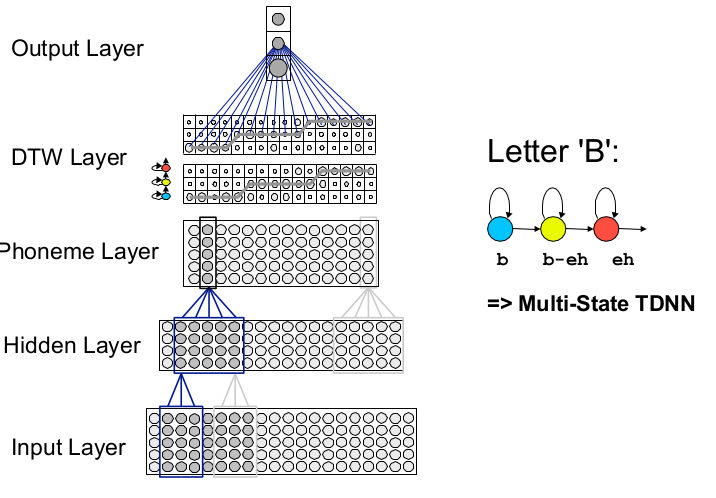
\includegraphics[scale=0.5]{MS-TDNN1}

Ich versuche die Distanz zwischen dem richtigen Wort und dem besten, falschem Wort zu maximieren. Das heißt wir optimieren die phonetische Sequenz und nicht die Wörter an sich.
Im MS-TDNN befindet sich ein Decoder. Das Alinieren der Zustände und der Feature, welche das neuronale Netz über die Zeit gelernt hat, läuft wie ein HMM mit dynamik time warping oder mit Viterbi Decoding. Der Unterschie dzu den Hypbriden, welche danach dran kommen, ist, dass das es sich hierbei um hidden Features handelt.

\subsubsection{NN-HMM Hybride}
Die Idee ist, dass ein neuronales Netz gebaut wird, welches die Phoneme erkennt. Wenn der Output statisch interpretiert werden kann, wird ein HMM Decoder obendrüber gebaut, der für das Alignment und die Integration der Wörter zuständig ist.
Die Wahrscheinlichkeit, welche wir als Output des NN bekommen, ist nicht die richige. Um die richige Wahrscheinlichkeit zu erhalten, müssen wir die Bayes Regel umformulieren. Wir wollen P(A|W) haben aber P(W|A).\\
Die (log)Wortwahrscheinlichkeit besteht aus der Summe der (log)Output Activations entlang des besten Pfades (bestimmt mit DTW oder Viterbi).

Kontextabhängige Phonemmodelle (a in Kontext von P etc.)

\subsubsection{Viterbi-Algorithmus}
\label{sssect:viterbi-algorithmus}
Der Viterbi Algorithmus sucht das beste Alignment zwischen allen phonetischen Sequenzen, die vorkommen können und der gesprochenen Sprache.
\subsubsection{Forward-Algorithmus}
\label{sssect:forward-algorithmus}

\subsubsection{Backward-Algorithmus}
\label{sssect:backward-algorithmus}

\newpage